\documentclass[../../main/main.tex]{subfiles}
\graphicspath{{./figures/}}

\dominitoc
\faketableofcontents

% \renewcommand{\mtcSfont}{\small\bfseries}
% \renewcommand{\mtcSSfont}{\footnotesize}
\mtcsettitle{minitoc}{}
\mtcsetrules{*}{off}

\makeatletter
\renewcommand{\@chapapp}{\'Electrocin\'etique -- chapitre}
\renewcommand{\chaplett}{E}
\makeatother

% \toggletrue{student}
% \toggletrue{corrige}
% \renewcommand{\mycol}{black}
% \renewcommand{\mycol}{gray}

\hfuzz=5.003pt

\begin{document}
\setcounter{chapter}{4}

\settype{book}
\settype{prof}
\settype{stud}

\chapter{Oscillateur amorti}

\vspace*{\fill}

\begin{tcn}(appl)<ctc>"somm"'t'{Sommaire}
	\let\item\olditem
	\vspace{-15pt}
	\minitoc
	\vspace{-25pt}
\end{tcn}

\begin{tcn}[sidebyside](appl)<ctb>"how"'t'{Capacités exigibles}
	\begin{itemize}[label=\rcheck]
		\item Analyser, sur des relevés expérimentaux, l'évolution de la forme des
		      régimes transitoires en fonction des paramètres caractéristiques.
		\item Prévoir l'évolution du système à partir de considérations
		      énergétiques.
		\item Écrire sous forme canonique l'équation différentielle afin
		      d'identifier la pulsation propre et le facteur de qualité.
		\item Décrire la nature de la réponse en fonction de la valeur du facteur
		      de qualité.
	\end{itemize}
	\tcblower
	\begin{itemize}[label=\rcheck]
		\item Caractériser l'évolution en utilisant les notions d'amplitude, de
		      phase, de période, de fréquence, de pulsation.
		\item Réaliser un bilan énergétique.
		\item Déterminer la réponse détaillée dans le cas d'un régime libre ou
		      d'un système soumis à un échelon en recherchant les racines du
		      polynôme caractéristique.
		\item Déterminer un ordre de grandeur de la durée du régime transitoire
		      selon la valeur du facteur de qualité.
	\end{itemize}
\end{tcn}

\vspace*{\fill}
\newpage
\vspace*{\fill}

%\vspace{-15pt}
\begin{tcn}[%
		sidebyside, fontupper=\small, fontlower=\small
	](appl)<ctb>"chek"'t'{L'essentiel}
	\begin{tcn}[nsp](defi)<ctc>'t'{Définitions}
		\vspace{-25pt}
		\tcblistof[\subsubsection*]{defi}{\hspace*{4.8pt}}
	\end{tcn}
	% \begin{tcn}[nsp](rapp)<ctc>'t'{Rappels}
	% 	\tcblistof[\subsubsection*]{rapp}{\hspace*{4.8pt}}
	% \end{tcn}
	\begin{tcn}[nsp](prop)<ctc>'t'{Propriétés}
		\vspace{-25pt}
		\tcblistof[\subsubsection*]{prop}{\hspace*{4.8pt}}
		% \tcblistof[\subsubsection*]{loi}{\hspace*{4.8pt}}
		% \tcblistof[\subsubsection*]{theo}{\hspace*{4.8pt}}
	\end{tcn}
	% \begin{tcn}[nsp](loi)<ctc>'t'{Lois}
	% 	\tcblistof[\subsubsection*]{loi}{\hspace*{4.8pt}}
	% \end{tcn}
	% \begin{tcn}[nsp](coro)<ctc>'t'{Corollaires}
	%   \tcblistof[\subsubsection*]{coro}{\hspace*{4.8pt}}
	% \end{tcn}
	% \begin{tcn}[nsp](demo)<ctc>'t'{Démonstrations}
	% 	\tcblistof[\subsubsection*]{demo}{\hspace*{4.8pt}}
	% 	\tcblistof[\subsubsection*]{prev}{\hspace*{4.8pt}}
	% \end{tcn}
	% \begin{tcn}[nsp](inte)<ctc>'t'{Interprétations}
	% 	\tcblistof[\subsubsection*]{inte}{\hspace*{4.8pt}}
	% \end{tcn}
	\begin{tcn}[nsp](impl)<ctc>'t'{Implications}
		\vspace{-25pt}
		\tcblistof[\subsubsection*]{impl}{\hspace*{4.8pt}}
	\end{tcn}
	% \begin{tcn}[nsp](tool)<ctc>'t'{Outils}
	% 	\tcblistof[\subsubsection*]{tool}{\hspace*{4.8pt}}
	% \end{tcn}
	% \begin{tcn}[nsp](nota)<ctc>'t'{Notations}
	% 	\tcblistof[\subsubsection*]{nota}{\hspace*{4.8pt}}
	% \end{tcn}
	% \begin{tcn}[nsp](appl)<ctc>'t'{Applications}
	% 	\tcblistof[\subsubsection*]{appl}{\hspace*{4.8pt}}
	% \end{tcn}
	% \begin{tcn}[nsp](rema)<ctc>'t'{Remarques}
	%   \tcblistof[\subsubsection*]{rema}{\hspace*{4.8pt}}
	% \end{tcn}
	% \begin{tcn}[nsp](exem)<ctc>'t'{Exemples}
	%   \tcblistof[\subsubsection*]{exem}{\hspace*{4.8pt}}
	% \end{tcn}
	% \begin{tcn}[nsp](ror)<ctc>"hart"'t'{Points importants}
	%   \tcblistof[\subsubsection*]{ror}{\hspace*{4.8pt}}
	% \end{tcn}
	% \begin{tcn}[nsp](impo)<ctc>'t'{Erreurs communes}
	%   \tcblistof[\subsubsection*]{impo}{\hspace*{4.8pt}}
	% \end{tcn}
	\tcblower
	% \begin{tcn}[nsp](defi)<ctc>'t'{Définitions}
	%   \tcblistof[\subsubsection*]{defi}{\hspace*{4.8pt}}
	% \end{tcn}
	% \begin{tcn}[nsp](rapp)<ctc>'t'{Rappels}
	%   \tcblistof[\subsubsection*]{rapp}{\hspace*{4.8pt}}
	% \end{tcn}
	% \begin{tcn}[nsp](prop)<ctc>'t'{Propriétés}
	% \tcblistof[\subsubsection*]{prop}{\hspace*{4.8pt}}
	% \tcblistof[\subsubsection*]{loi}{\hspace*{4.8pt}}
	% \tcblistof[\subsubsection*]{theo}{\hspace*{4.8pt}}
	% \end{tcn}
	% \begin{tcn}[nsp](coro)<ctc>'t'{Corollaires}
	%   \tcblistof[\subsubsection*]{coro}{\hspace*{4.8pt}}
	% \end{tcn}
	\begin{tcn}[nsp](inte)<ctc>'t'{Interprétations}
		\vspace{-25pt}
		\tcblistof[\subsubsection*]{inte}{\hspace*{4.8pt}}
	\end{tcn}
	\begin{tcn}[nsp](demo)<ctc>'t'{Démonstrations}
		\vspace{-25pt}
		\tcblistof[\subsubsection*]{demo}{\hspace*{4.8pt}}
		% \tcblistof[\subsubsection*]{prev}{\hspace*{4.8pt}}
	\end{tcn}
	% \begin{tcn}[nsp](inte)<ctc>'t'{Interprétations}
	% 	\tcblistof[\subsubsection*]{inte}{\hspace*{4.8pt}}
	% \end{tcn}
	% \begin{tcn}[nsp](impl)<ctc>'t'{Implications}
	% 	\tcblistof[\subsubsection*]{impl}{\hspace*{4.8pt}}
	% \end{tcn}
	% \begin{tcn}[nsp](tool)<ctc>'t'{Outils}
	%   \tcblistof[\subsubsection*]{tool}{\hspace*{4.8pt}}
	% \end{tcn}
	% \begin{tcn}[nsp](nota)<ctc>'t'{Notations}
	% 	\tcblistof[\subsubsection*]{nota}{\hspace*{4.8pt}}
	% \end{tcn}
	% \begin{tcn}[nsp](odgr)<ctc>'t'{Ordres de grandeur}
	% 	\tcblistof[\subsubsection*]{odgr}{\hspace*{4.8pt}}
	% \end{tcn}
	% \begin{tcn}[nsp](appl)<ctc>'t'{Applications}
	% 	\tcblistof[\subsubsection*]{appl}{\hspace*{4.8pt}}
	% \end{tcn}
	% \begin{tcn}[nsp](rema)<ctc>'t'{Remarques}
	%   \tcblistof[\subsubsection*]{rema}{\hspace*{4.8pt}}
	% \end{tcn}
	% \begin{tcn}[nsp](exem)<ctc>'t'{Exemples}
	% 	\tcblistof[\subsubsection*]{exem}{\hspace*{4.8pt}}
	% \end{tcn}
	\begin{tcn}[nsp](ror)<ctc>"hart"'t'{Points importants}
		\vspace{-25pt}
		\tcblistof[\subsubsection*]{ror}{\hspace*{4.8pt}}
	\end{tcn}
	% \begin{tcn}[nsp](impo)<ctc>'t'{Erreurs communes}
	% 	\tcblistof[\subsubsection*]{impo}{\hspace*{4.8pt}}
	% \end{tcn}
\end{tcn}

\vspace*{\fill}

\newpage

\section{Introduction}

\subsection{Évolutions en régime libre, exemple RLC}

\begin{minipage}{0.60\linewidth}
	En reprenant les résultats du LC libre, nous devrions en réalité observer que
	les oscillations dans le circuit s'atténuent. Soit le circuit RLC
	suivant\ftn{\url{https://tinyurl.com/ypbwcwfs}}, avec $L = \SI{43}{mH}$ et $C
		= \SI{20}{nF}$~:
\end{minipage}
\begin{minipage}{0.40\linewidth}
	\begin{center}
		\sswitch{%
			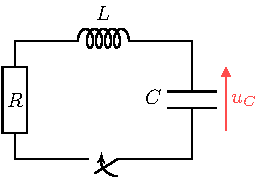
\includegraphics[width=.7\linewidth, draft=true]{rlc_descendant}
		}{%
			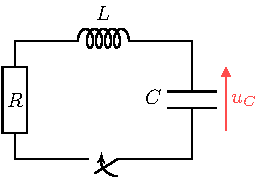
\includegraphics[width=.7\linewidth]{rlc_descendant}
		}%
		\vspace{-15pt}
		\captionof{figure}{}
	\end{center}
\end{minipage}

\begin{itemize}
	\item Lorsque la \textbf{résistance est petite}~: on observe \textbf{plusieurs
		      oscillations}.
	      \bigbreak
	      On observe une série d'oscillations à la période $T \approx
		      \SI{184}{\micro s}$. On observe environ 15 oscillations lorsque $R
		      \approx \SI{100}{\ohm}$ (résistance interne du GBF + de la bobine), 9
	      oscillations lorsque $R \approx \SI{180}{\ohm}$, 3 oscillations lorsque
	      $R \approx \SI{500}{\ohm}$.
\end{itemize}
\begin{minipage}{0.45\linewidth}
	\begin{center}
		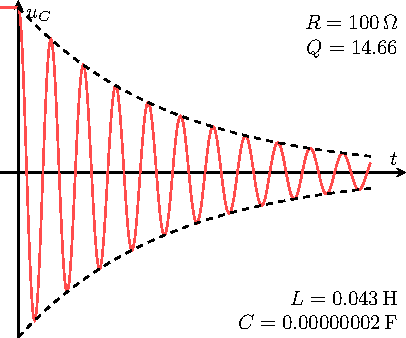
\includegraphics[width=.7\linewidth]{carac-rlc-15}
	\end{center}
\end{minipage}
\hfill
\begin{minipage}{0.45\linewidth}
	\begin{center}
		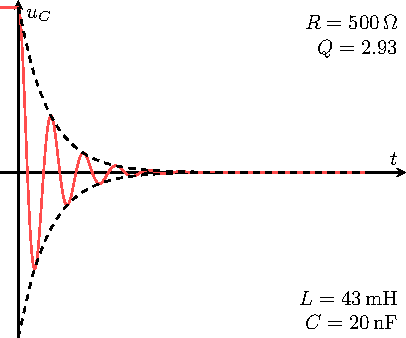
\includegraphics[width=.7\linewidth]{carac-rlc-3}
	\end{center}
\end{minipage}

\begin{itemize}
	\item Lorsque la \textbf{résistance est plus grande}~: les
	      \textbf{oscillations disparaissent}.
	      \bigbreak
	      Lorsque $R \approx \SI{2,9}{k\ohm}$, on
	      observe un régime transitoire dont la durée est d'environ
	      $\SI{250}{\micro s}$ (à 95\%). Lorsque $R \approx \SI{7.5}{k\ohm}$, on
	      observe un régime transitoire plus long, d'environ \SI{420}{\micro s}.
\end{itemize}
\begin{minipage}{0.45\linewidth}
	\begin{center}
		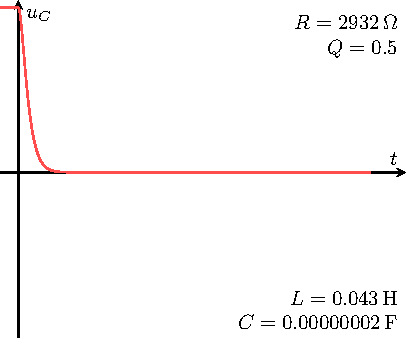
\includegraphics[width=.7\linewidth]{carac-rlc-05}
	\end{center}
\end{minipage}
\hfill
\begin{minipage}{0.45\linewidth}
	\begin{center}
		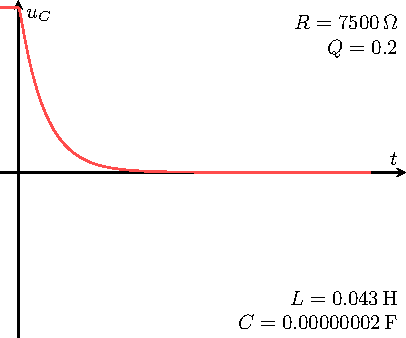
\includegraphics[width=.7\linewidth]{carac-rlc-02}
	\end{center}
\end{minipage}

\begin{tcn}(obsv)<lftt>{Analyse}
	Lorsque l'on excite le système RLC, le système a deux principales réponses~:
	\begin{enumerate}
		\item[b]{Système oscillant} pour $R < R_{c}$, de pseudo-période\ftn{On parle
			      de \textit{pseudo}-période car le signal est diminué.}
		      \textbf{supérieure à $T_0$}~;
		\item[b]{Système non-oscillant} pour $R > R_c$~: le transitoire
		      \textbf{augmente avec $R$}.
	\end{enumerate}
\end{tcn}

\subsection{Équation différentielle}

\begin{tcb}[label=prop:eqdiffoh](prop){Équation différentielle amorti}
	Un oscillateur amorti à un degré de liberté est un système dont l'évolution
	temporelle est décrite par une grandeur $x(t)$ solution d'un équation
	différentielle du type~:
	\psw{%
	\[
		\boxed{
		\dv[2]{x}{t} + \frac{\w_0}{Q} \dv{x}{t} + \w_0{}^2x =
		\w_0{}^2x_{\rm eq}
		}%
	\]
	}%
	\vspace{-15pt}
	\begin{tasks}[label=\arabic*)](3)
		\task $x_{\rm eq}$ la position d'équilibre
		\task $\w_0$ la pulsation \textbf{propre}
		\task $Q$ le \textbf{facteur de qualité}
	\end{tasks}
\end{tcb}

\begin{tcb}[label=rema:eqdiffamorti](rema)<lftt>{Analyse de l'équation}
	Par lecture de cette équation, $Q$ est \textbf{sans dimension} pour qu'on
	retrouve que $\w_0$ s'exprime en \si{s^{-1}} car $\dv{x}{t}$ est de dimension
	$[x]\cdot\si{s^{-1}}$.
	\bigbreak
	De plus, on remarque que \textbf{plus $Q$ est élevé}, plus le terme
	d'ordre 1 est négligeable devant les autres, donc \textbf{plus on se
		rapproche de l'harmonique}. Le \textbf{facteur de qualité} traduit donc à
	quel point le système est \textbf{idéal}.
\end{tcb}

\subsection{Équation caractéristique et régimes de solutions}
\begin{tcb*}[label=def:eqcarac, sidebyside]
	(defi){Équation caractéristique amorti}
	Pour résoudre une équation différentielle \textbf{homogène}, on suppose une
	solution de la forme $x(t) = A\exp(rt)$ avec $r \in \Cb$. En injectant cette
	expression dans l'équation différentielle, on obtient l'\textbf{équation
		caractéristique}~:
	\psw{%
		\begin{equation*}
			\boxed{r^2 + \frac{\w_0}{Q}r + \w_0{}^2 = 0}
		\end{equation*}
	}%
	\tcblower
	C'est un trinôme du second degré, dont le discriminant $\Delta$ est
	\psw{%
		\begin{equation*}
			\boxed{
				\Delta =
				\left( \frac{\w_0}{Q} \right)^2 - 4\w_0{}^2 =
				\frac{\w_0{}^{2}}{Q^{2}}\left( 1-4Q^{2} \right)
			}%
		\end{equation*}
	}%
\end{tcb*}

\begin{tcb*}[label=impl:eqcarac](impl){Régimes de solutions}
	Selon la valeur du discriminant, on aura différentes valeurs de $r$~:
	%  , doubles
	% réelles, simple réelle ou doubles complexes. On a en effet
	\psw{%
		\begin{gather*}
			\Delta > 0
			\Lra
			\cancel{\frac{\w_0{}^{2}}{Q^{2}}}\left( 1-4Q^{2} \right) >0
			\Lra
			4Q^2 < 1
			\Lra
			Q < \frac{1}{2}
		\end{gather*}
	}%
	\vspace{-15pt}
	\begin{description}
		\item{}[$\mathbf{Q > 1/2}$] :
		      \psw{%
			      régime \textbf{pseudo-périodique},
			      racines complexes et oscillations décroissantes~;
		      }%
		\item{}[$\mathbf{Q = 1/2}$] :
		      \psw{%
			      régime \textbf{critique}, racine double
			      réelle~;
		      }%
		\item{}[$\mathbf{Q < 1/2}$] :
		      \psw{%
			      régime \textbf{apériodique}, racines
			      réelles et décroissance exponentielle sans oscillation.
		      }%
	\end{description}
\end{tcb*}

\begin{tcb}[label=nota:pm](nota)<lftt>{$\pm$ et $\mp$}
	Il est courant de noter les racines $r_\pm$ pour dénoter à la fois $r_+$ et
	$r_-$. Dans ce cas, l'expression de la racine contient le signe $\pm$, ce
	qui signifie que $r_+$ correspond à l'expression avec le $+$, et $r_-$
	correspond à l'expression avec le $-$.
	\smallbreak
	Si l'expression contient le signe $\mp$, c'est l'opposé~: $r_+$ correspond à
	l'expression avec $-$.
\end{tcb}

% \begin{tcb}[label=prop:solureg, tabularx={Y|Y|Y}]
% 	(ror){Solutions oscillateur amorti}
% 	\vspace{8pt}
% 	\textbf{Pseudo-périodique} &
% 	\vspace{8pt}
% 	\textbf{Critique} &
% 	\vspace{8pt}
% 	\textbf{Apériodique}
% 	\\\hline
% 	$\D < 0 \Lra Q > 1/2$ & $\D = 0 \Lra Q = 1/2$ & $\D >
% 		0 \Lra Q < 1/2$
% 	\\\hline
% 	\begin{equation*}
% 		\boxed{r_\pm = - \frac{\w_0}{2Q} \pm \jj\W}
% 	\end{equation*}
% 	\begin{equation*}
% 		\boxed{\W = \frac{\w_0}{2Q}\sqrt{4Q^2 - 1}}
% 	\end{equation*}
% 	&
% 	\begin{equation*}
% 		\boxed{r = - \frac{\w_0}{2Q} = -\w_0}
% 	\end{equation*}
% 	&
% 	\begin{equation*}
% 		\boxed{r_\pm = \frac{\w_0}{2Q}\left(-1 \pm \sqrt{1 - 4Q^2}\right)}
% 	\end{equation*}
% 	\\\hline
% 	\begin{empheq}[box=\fbox]{gather*}
%     x(t) = \underbracket[1pt]{\exp \left(-\frac{\w_0}{2Q}t\right)}_{
% 			\text{partie décroissante}}\times\\
%       \underbracket[1pt]{\left[ A\cos(\Wt) + B\sin(\Wt) \right]}_{
% 			\text{partie oscillante}}
% 	\end{empheq}
% 	&
% 	\begin{equation*}
% 		\boxed{x(t) = (At + B)\exp(-\w_0t)}
% 	\end{equation*}
% 	&
% 	\begin{empheq}[box=\fbox]{gather*}
% 		x(t) = A\exp(r_+t) +\\
% 		\hspace{26pt} B\exp(r_-t)
% 	\end{empheq}
% 	\\
% \end{tcb}
\begin{tcb}[label=prop:solureg, tabularx={l|Y|Y}]
	(ror){Solutions oscillateur amorti}
	&
	\vspace{8pt}
	\textbf{Racines} &
	\vspace{8pt}
	\textbf{Solution}
	\\\hline
	\rotatebox[origin=c]{90}{%
		\hspace{8pt}
		% $\D < 0 \Lra Q > 1/2$
		\textbf{Pseudo-pér.}
		\hspace{8pt}
	}
	&
	\begin{align*}
		r_\pm = - \frac{\w_0}{2Q} \pm \jj\W
		\qav
		\W    = \frac{\w_0}{2Q}\sqrt{4Q^2 - 1}
	\end{align*}
	&
	\begin{gather*}
		x(t) = \underbracket[1pt]{
			\exp \left(-\frac{\w_0}{2Q}t\right)
		}_{
			\text{partie décroissante}
		}\times
		\underbracket[1pt]{
			\left[ A\cos(\Wt) + B\sin(\Wt) \right]
		}_{
			\text{partie oscillante}
		}
	\end{gather*}
	\\\hline
	\rotatebox[origin=c]{90}{%
		\hspace{8pt}
		% $\D = 0 \Lra Q = 1/2$
		\textbf{Critique}
		\hspace{8pt}
	}
	&
	\begin{equation*}
		r = - \frac{\w_0}{2Q} = -\w_0
	\end{equation*}
	&
	\begin{equation*}
		x(t) = (At + B)\exp(-\w_0t)
	\end{equation*}
	\\\hline
	\rotatebox[origin=c]{90}{%
		\hspace{8pt}
		% $\D > 0 \Lra Q < 1/2$
		\textbf{Apériodique}
		\hspace{8pt}
	}
	&
	\begin{equation*}
		r_\pm = \frac{\w_0}{2Q}\left(-1 \pm \sqrt{1 - 4Q^2}\right)
	\end{equation*}
	&
	\begin{gather*}
		x(t) = A\exp(r_+t) + B\exp(r_-t)
	\end{gather*}
	\\
\end{tcb}

\section{Oscillateur amorti électrique~: circuit RLC série libre}
\subsection{Présentation}

\begin{tcb*}[sidebyside, righthand ratio=.30](defi){Circuit RLC libre}
	\begin{itemize}
		\item Il est constitué de l'association en série d'une résistance, d'une
		      bobine et d'un condensateur idéaux.
		\item \textbf{On suppose le condensateur initialement chargé}.
		      % ~:
		      %   \fbox{$u_C(0^-) = E$ \underline{et} $i(0^-) = 0$} (condensateur chargé
		      %   $\equiv$ interrupteur ouvert).
		\item À $t=0$, on coupe le générateur.
	\end{itemize}
	\tcblower
	\begin{center}
		\sswitch{%
			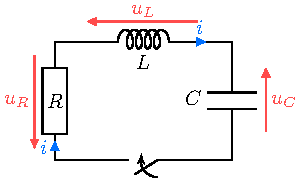
\includegraphics[width=.9\linewidth, draft=true]{rlc_descendant-intens}
		}{%
			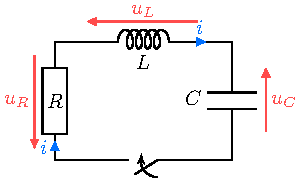
\includegraphics[width=.9\linewidth]{rlc_descendant-intens}
		}%
		\captionof{figure}{}
	\end{center}
\end{tcb*}

\subsection{Bilan énergétique}
\begin{tcb*}[label=demo:rcenerg-charge](demo){Bilan de puissance RLC libre}
	On fait un bilan de puissances~:
	\psw{%
		\begin{DispWithArrows*}[fleqn, mathindent=10pt]
			u_Ci + u_Li + u_Ri &= 0
			\Arrow{$i = C \dv{u_C}{t}$, $u_L = L \dv{i}{t}$ et $u_R = Ri$}
			\\\Lra
			u_C\times C \dv{u_C}{t} + L \dv{i}{t}\times i + Ri^2 &= 0
			\Arrow{$\Pc_J = Ri^{2}$ et $f \times f' = \left(\frac{1}{2}f^{2}\right)'$}
			\\\Lra
			\dv{}{t}
			\Big(
			\underbracket[1pt]{\frac{1}{2}C  u_C{}^2}_{\Ec_C} +
			\underbracket[1pt]{\frac{1}{2}Li^2}_{\Ec_L}
			\Big) &= -\Pc_J
		\end{DispWithArrows*}
	}%
	\vspace{-15pt}
\end{tcb*}
\begin{tcb*}[label=prop:lcenerg-décharge](prop){Bilan de puissance RLC libre}
	L'énergie emmagasinée dans le circuit est progressivement dissipée par
	effet \textsc{Joule} dû à la résistance~:
	\psw{%
		\[
			\boxed{\dv{\Ec}{t} = -\Pc_J}
		\]
	}%
	avec $\Ec = \Ec_C + \Ec_L = \frac{1}{2}Cu_C{}^2 + \frac{1}{2}Li^2$.
\end{tcb*}
\begin{tcb}[label=ror:amortissement, cnt, bld]
	(ror)<lftt>{Évolution énergétique RLC série}
	On a donc bien une perte d'énergie à cause de la dissipation dans la
	résistance. Il y aura donc progressivement une perte de la tension
	de $u_C$, d'où l'amortissement.
\end{tcb}

\subsection{Équation différentielle du circuit}
\begin{tcb*}[label=demo:eqdiffrc, sidebyside, sidebyside align=top]
	(demo)<lftt>{Équation différentielle RLC libre}
	Avec la loi des mailles,
	\psw{%
		\begin{DispWithArrows*}[fleqn, mathindent=2pt]
			u_L + u_R + u_C &= 0
			\Arrow{$u_L = L \dv{i}{t}$\\et $u_R = Ri$}
			\\\Lra
			L \dv{i}{t} + Ri + u_C &= 0
			\Arrow{$i = C \dv{u_C}{t}$}
			\\\Lra
			LC \dv[2]{u_C}{t} + RC \dv{u_C}{t} + u_C                   &= 0
			\Arrow{forme\\canonique}
			\\
			\Lra \dv[2]{u_C}{t} + \frac{R}{L} \dv{u_C}{t} + \frac{1}{LC}u_C &= 0
		\end{DispWithArrows*}
	}%
	\vspace{-30pt}
	\tcblower
	On détermine l'expression de $Q$ par identification~:
	\psw{%
		\begin{DispWithArrows*}
			\frac{\w_0}{Q} &= \frac{R}{L}
			\Arrow{$\w_0 = \frac{1}{\sqrt{LC}}$}
			\\\Lra
			\frac{1}{Q \sqrt{LC}} &= \frac{R}{L}
			\Arrow{On isole $Q$}
			\\\Lra
			Q &= \frac{L}{R \sqrt{LC}}
			\Arrow{$L = \sqrt{L}^{2}$}
			\\\Lra
			\Aboxed{Q &= \frac{1}{R}\sqrt{\frac{L}{C}}}
		\end{DispWithArrows*}
	}%
	\vspace{-30pt}
\end{tcb*}

\begin{tcb*}[label=prop:eqdiffrc, sidebyside, righthand ratio=.4]
	(prop){Équation différentielle RLC libre}
	L'équation différentielle de la tension $u_C(t)$ aux bornes d'un
	condensateur d'un circuit RLC en régime libre est
	\psw{%
		\[
			\boxed{\dv[2]{u_C}{t} + \frac{\w_0}{Q} \dv{u_C}{t} + \w_0{}^2u_C = 0}
		\]
	}%
	\begin{itemize}
		\item
		      \psw{%
			      $\DS\boxed{\w_0 = \frac{1}{\sqrt{LC}}}$ la pulsation propre~;
		      }%
		\item
		      \psw{%
			      $\DS\boxed{Q = \frac{1}{R} \sqrt{\frac{L}{C}}}$ le facteur de
			      qualité.
		      }%
	\end{itemize}
	\tcblower
	Les conditions initiales (continuité de $u_C$ aux bornes de $C$
	et de $i$ traversant $L$) sont
	\psw{%
		\begin{empheq}[box=\fbox]{align*}
			u_C(0^-) &= u_C(0^+) = E\\
			i(0^-) &= i(0^+) = 0
		\end{empheq}
	}%
\end{tcb*}

\subsection{Résolutions pour chaque cas}
\subsubsection{Cas $\D < 0 \Lra Q > 1/2$~: régime pseudo-périodique}
\paragraph{Solution de l'équation}
~ \smallbreak

\begin{tcb*}[label=demo:solupseudoper, breakable]
	(demo){Solution pseudo-périodique}
	On part de l'équation caractéristique~:
	\[
		\psw{%
			r^{2} + \frac{\w_0}{Q}r + \w_0{}^{2} = 0
		}%
		\qdc
		\psw{%
			\Delta = \frac{\w_0{}^{2}}{Q^{2}}\left( 1-4Q^{2} \right) < 0
		}%
	\]
	Ainsi,
	\vspace{-25pt}
	\psw{%
		\begin{DispWithArrows*}
			r_\pm & = \frac{-\frac{\w_0}{Q} \pm \jj\sqrt{-\D}}{2}
			\Arrow{On injecte $\Delta$}
			\\\Lra
			r_\pm &= -\frac{\w_0}{2Q} \pm
			\frac{\jj}{2} \sqrt{\frac{\w_0{}^{2}}{Q^{2}}\left( 4Q^{2}-1 \right)}
			\Arrow{On extrait $\frac{\w_0}{Q}$}
			\\\Lra
			r_\pm &= - \frac{\w_0}{2Q} \pm \jj \frac{\w_0}{2Q} \sqrt{4Q^{2}-1}
			\Arrow{On définit $\W$}
			\\\Lra
			r_\pm &= - \frac{\w_0}{2Q} \pm \jj\W
		\end{DispWithArrows*}
	}%
	\vspace{-15pt}
	\begin{gather*}
		\beforetext{d'où la définition de $\W$~:}
		\boxed{\W = \frac{\w_0}{2Q}\sqrt{4Q^{2}-1}}
	\end{gather*}
	Ensuite, avec la forme générale de la solution on a
	\psw{%
		\begin{equation*}
			u_C(t) = \exp \left(-\frac{\w_0}{2Q}t\right)
			\left[ A\cos(\Wt) + B\sin(\Wt) \right]
		\end{equation*}
	}%
	\vspace{-15pt}
	\begin{itemize}
		\item On trouve $A$ avec la première condition initiale~:
		      \psw{%
			      \begin{gather*}
				      u_C(0) = E = 1 \left[ A \cdot 1 + B \cdot 0 \right] = A
				      \quad \Ra \quad \boxed{A=E}
			      \end{gather*}
		      }%
		      \vspace{-25pt}
		\item On trouve $B$ avec la seconde CI~:
		      \psw{%
			      \begin{gather*}
				      \hspace*{-10pt}
				      \dv{u_C}{t} =
				      -\frac{\w_0}{2Q}\exp \left( -\frac{\w_0}{2Q}t \right)\times
				      \left[ A\cos(\Wt) + B\sin(\Wt) \right] +
				      \exp \left( -\frac{\w_0}{2Q}t \right)
				      \left[ -A\W\sin(\Wt) + B\W\cos(\Wt) \right]
				      \\\Ra
				      \qty(\dv{u_C}{t})_0 = - \frac{\w_0}{2Q}A + \W B = 0
				      \Lra
				      \boxed{B = \frac{\w_0}{2Q\W}E = \frac{E}{\sqrt{4Q^2-1}}}
			      \end{gather*}
		      }%
		      % \vspace{-15pt}
	\end{itemize}
	% Ainsi, on trouve bien
	% \begin{empheq}[box=\fbox]{gather*}
	% 	u_C(t) = E\exp \left( -\frac{\w_0}{2Q}t \right)\times
	% 	\left[
	% 		\cos(\Wt) + \frac{1}{\sqrt{4Q^2 - 1}}\sin(\Wt)
	% 		\right]
	% \end{empheq}
\end{tcb*}
\begin{tcb*}[label=prop:solupseudoper, sidebyside, righthand ratio=.3]
	(prop){Solution pseudo-périodique}
	Pour un facteur de qualité $Q > 1/2$, $u_C$ s'exprime par
	\psw{%
		\begin{empheq}[box=\fbox]{gather*}
			u_C(t) = E\exp \left( -\frac{\w_0}{2Q}t \right)\times
			\left[
				\cos(\Wt) + \frac{1}{\sqrt{4Q^2 - 1}}\sin(\Wt)
				\right]
		\end{empheq}
	}%
	\vspace{-15pt}
	\begin{gather*}
		\beforetext{avec}
		\W = \frac{\sqrt{-\Delta}}{2}
		\Lra
		\boxed{\W = \frac{\w_0}{2Q} \sqrt{4Q^2 - 1}}
	\end{gather*}
	La période des oscillations est alors
	% \textbf{diffère des oscillations harmoniques} $T_0
	% = 2\pi/\w_0$ selon
	\psw{%
		\begin{equation*}
			T =
			\frac{2\pi}{\W} =
			\frac{2\pi}{\w_0} \frac{2Q}{\sqrt{4Q^{2} - 1}}
			\Lra
			\boxed{T = T_0 \frac{2Q}{\sqrt{4Q^2-1}} > T_0}
		\end{equation*}
	}%
	\tcblower
	% Les oscillations se font entre les courbes
	Les enveloppes sont
	\[y(t) = \pm E \exp \left( - \frac{\w_0}{2Q}t \right)\]
	\begin{center}
		\sswitch{%
			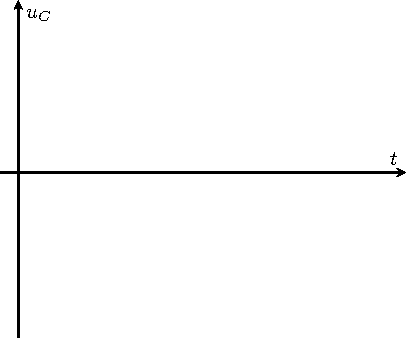
\includegraphics[width=\linewidth]{carac-rlc_empty}
		}{%
			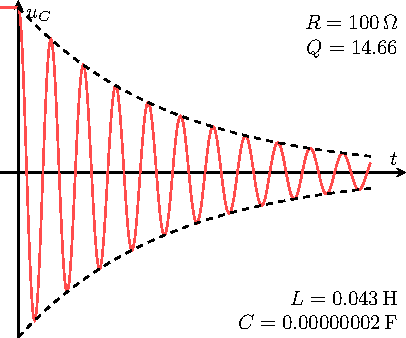
\includegraphics[width=\linewidth]{carac-rlc-15}
		}%
		\captionof{figure}{}
	\end{center}
\end{tcb*}

\begin{tcb*}[breakable](inte){Résultat pseudo-périodique}
	La solution du polynôme caractéristique s'écrit donc comme la \textbf{somme
		de la solution d'ordre 1 et de la solution d'ordre 2 harmonique}~:
	\psw{%
		\begin{gather*}
			r_{\pm} =
			\xunderbracket{-\frac{\w_0}{2Q}}_{\equiv -\frac{1}{\tau}}
			\pm
			\xunderbracket{\jj \Omega}_{\equiv \jw}
			\qso
			\boxed{r_{\pm} = r\ind{ordre 1} + r\ind{ordre 2 harmonique}}
		\end{gather*}
	}%
	Ceci n'est pas très étonnant puisque l'EDLHC d'ordre 2 amortie est la somme
	d'une EDLHC d'ordre 2 harmonique et d'une EDLHC d'ordre 1.
	\tcblower
	Avec les propriétés de l'exponentielle ($\exr^{a+b} = \exr^{a}\exr^{b}$), il
	est donc naturel que la solution amortie soit le \textbf{produit} des
	solutions d'ordre 1 et d'ordre 2~:
	\psw{%
		\begin{gather*}
			y_h(t) =
			\xunderbracket{\exp\left( -\frac{\w_0}{2Q}t \right)}_{\equiv
				\exr^{-t/\tau}}
			\xunderbracket{%
				\left[A\cos(\Omega t) + B\sin(\Omega t)\right]%
			}_{\equiv A\cos(\w_0t) + B\sin(\w_0t)}
			\qso
			\boxed{%
				y_h(t) = y_{h, \text{ordre 1}} \times y_{h, \text{ordre 2 harmonique}}
			}
		\end{gather*}
	}%
	\vspace{-15pt}
\end{tcb*}

\paragraph{Régime transitoire}
~ \smallbreak

\begin{tcb*}[label=demo:transipseudo](demo){Régime transitoire pseudo-pér.}
	L'amplitude varie selon $E\exp \DS \left( -\frac{\w_0}{2Q}t \right)$~; on
	définit donc $t_{95}$ tel que
	\psw{%
		\begin{DispWithArrows*}[fleqn, mathindent=10pt]
			\exp \left(-\frac{\w_0}{2Q}t_{95} \right) &= 0.05
			\CArrow{$\ln (\cdot)$}
			\\\Lra
			- \frac{\w_0}{2Q}t_{95} &= \ln(0.05)
			\Arrow{$0.05 = 1/20$ et $\ln (a^{b}) = b \ln a$}
			\\\Lra
			\frac{\w_0}{2Q}t_{95} &= \ln(20)
			\Arrow{On isole et $2 \ln 20 \approx 2\pi$}
			\\\Lra
			t_{95} &= 2\ln(20) \frac{Q}{\w_0} \approx \frac{2\pi}{\w_0}Q
		\end{DispWithArrows*}
	}%
\end{tcb*}

\begin{tcb*}[label=prop:transipseudo](prop){Régime transitoire $Q > 1/2$}
	Le temps de réponse à 95\% est atteint à partir de $t_{95}$ tel que
	\psw{%
		\begin{equation*}
			\boxed{t_{95} \approx QT_0} \qav \boxed{T_0 = \frac{2\pi}{\w_0}}
		\end{equation*}
	}%
	\vspace{-15pt}
\end{tcb*}

\begin{tcb}[label=impl:pseudograndQ](impl){Résultat à grand $Q$}
	Avec ces résultats on remarque en effet que quand $Q \rightarrow \infty$, on
	a à la fois
	\begin{equation*}
		\boxed{\W \approx \w_0} \qdc \boxed{T \approx T_0}
	\end{equation*}
	Mais aussi
	\begin{equation*}
		\boxed{\dv[2]{u_C}{t} + \w_0{}^2u_C = 0} \qdc \boxed{u_C(t) = E\cos(\w_0t)}
	\end{equation*}
	On retrouve toutes les caractéristiques de la situation harmonique.
\end{tcb}

\begin{tcb}[breakable](inte)<lftt>"bulb"{Espace des phases pseudo-pér.}
	Contrairement à la situation harmonique, le tracé de la solution dans
	l'espace $(u_C,i)$ n'est \textbf{pas symétrique par inversion du temps}~: la
	dissipation par effet \textsc{Joule} diminue l'énergie du système, et la
	\textbf{tension diminue progressivement}.
	\bigbreak
	On observera donc une \textbf{spirale décroissante} avec beaucoup
	d'oscillations quand les amortissements ne sont pas trop élevés, et de moins
	en moins quand $Q$ diminue.
	% ou que l'amortissement augmente.
	\tcblower
	\noindent
	\begin{minipage}{0.49\linewidth}
		\begin{center}
			\sswitch{%
				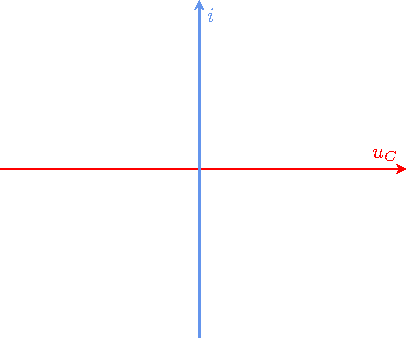
\includegraphics[width=.6\linewidth]{carac-rlc_xy-empty}
			}{%
				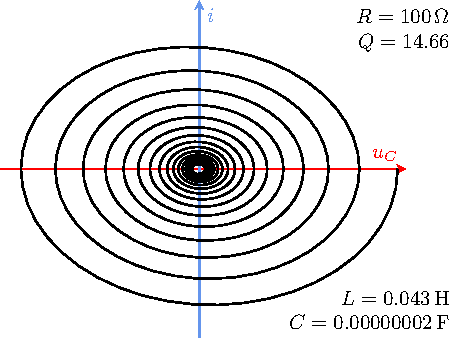
\includegraphics[width=.7\linewidth]{carac-rlc_xy-15}
			}%
			\captionof{figure}{Faible amortissement}
		\end{center}
	\end{minipage}
	\begin{minipage}{0.49\linewidth}
		\begin{center}
			\sswitch{%
				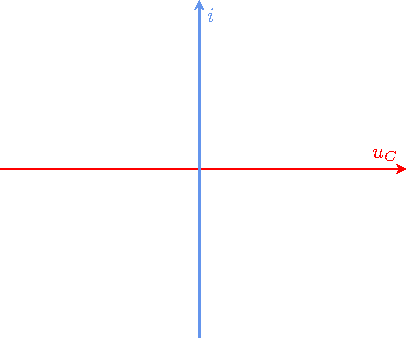
\includegraphics[width=.6\linewidth]{carac-rlc_xy-empty}
			}{%
				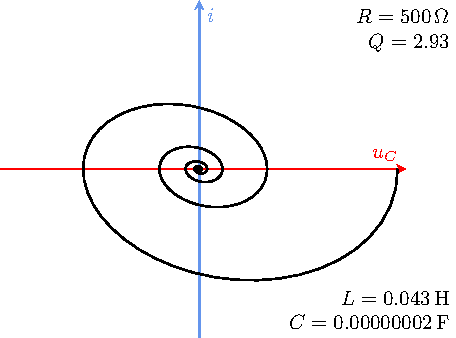
\includegraphics[width=.7\linewidth]{carac-rlc_xy-3}
			}%
			\captionof{figure}{Moyen amortissement}
		\end{center}
	\end{minipage}
\end{tcb}

% \newpage
\subsubsection{Cas $\D = 0 \Lra Q = 1/2$~: régime critique}
\paragraph{Solution de l'équation}
~\smallbreak

% \vspace{-15pt}
\begin{tcb*}[label=demo:solupseudoper](demo){Solution critique}
	La seule racine de l'équation caractéristique est double, et vaut
	\[
		\psw{%
			r = -\w_0
		}%
		\qso
		\psw{%
			u_C(t) = (At+B)\exp \left(-\w_0t\right)
		}%
	\]
	\vspace{-20pt}
	\begin{itemize}
		\item On trouve $B$ avec la première condition initiale~:
		      \psw{%
			      \begin{gather*}
				      u_C(0) = E = (A\cdot0 + B)\cdot1 = B
				      \quad \Ra \quad \boxed{B=E}
			      \end{gather*}
		      }%
		      \vspace{-15pt}
		\item On trouve $A$ avec la seconde CI~:
		      \psw{%
			      \begin{gather*}
				      \dv{u_C}{t} = (A)\exp(-\w_0t) +
				      (At+E)(-\w_0)\exp(-\w_0t)
				      \\\Ra
				      \qty(\dv{u_C}{t})_0 = A -\w_0E = 0
				      \Lra
				      \boxed{A = \w_0E}
			      \end{gather*}
		      }%
		      \vspace{-15pt}
	\end{itemize}
\end{tcb*}

\begin{tcb*}[label=prop:solupseudoper, sidebyside, righthand ratio=.3]
	(prop){Solution critique}
	Pour un facteur de qualité $Q = 1/2$, $u_C$ s'exprime par
	\psw{%
		\begin{empheq}[box=\fbox]{gather*}
			u_C(t) = E(\w_0t + 1) \exp(-\w_0t)
		\end{empheq}
	}%
	et on n'observe \textbf{pas une oscillation}.
	\tcblower
	\begin{center}
		\sswitch{%
			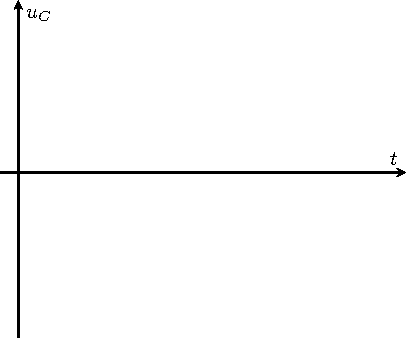
\includegraphics[width=\linewidth]{carac-rlc_empty}
		}{%
			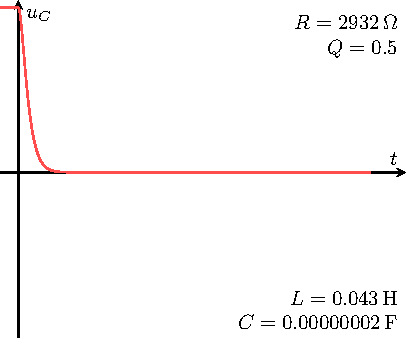
\includegraphics[width=\linewidth]{carac-rlc-05}
		}%
		\vspace{-15pt}
		\captionof{figure}{}
	\end{center}
\end{tcb*}

\begin{tcb}[sidebyside, righthand ratio=.3]
	(inte)<lftt>"bulb"{Espace des phases critique}
	Au facteur de qualité critique, l'amortissement est suffisamment important
	pour empêcher $u_C$ de passer sous 0.
	\tcblower
	\begin{center}
		\sswitch{%
			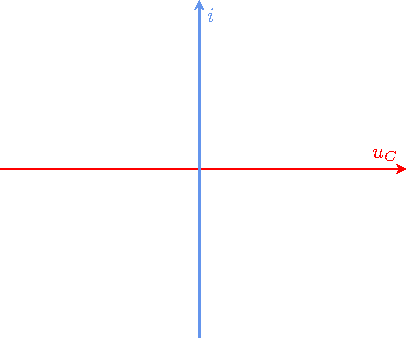
\includegraphics[width=.9\linewidth]{carac-rlc_xy-empty}
		}{%
			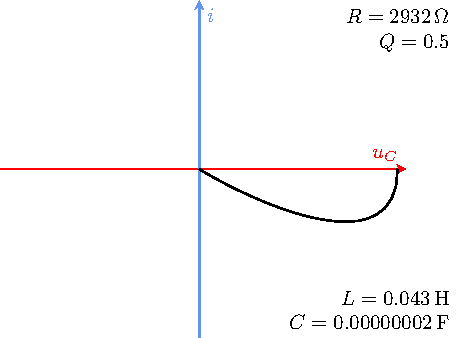
\includegraphics[width=.9\linewidth]{carac-rlc_xy-05}
		}%
		\captionof{figure}{}
	\end{center}
\end{tcb}

\paragraph{Régime transitoire}
~ \smallbreak

\begin{tcb*}[label=demo:transicrit](demo){Régime transitoire critique}
	En négligeant le terme linéaire en $t$ devant la décroissance
	exponentielle, on a
	\psw{%
		\begin{gather*}
			\exp (-\w_0t_{95}) = \num{0.05}
			\Lra
			t_{95} =
			\frac{\ln(20)}{\w_0}
			\approx
			\frac{\pi}{\w_0}
		\end{gather*}
	}%
	\vspace{-15pt}
\end{tcb*}
\begin{tcb*}[label=prop:transicrit](prop){Régime transitoire critique}
	Le temps de réponse à 95\% est atteint à partir de $t_{95}$ tel que
	\psw{%
		\begin{equation*}
			\boxed{t_{95} \approx \frac{T_0}{2}} \qav \boxed{T_0 = \frac{2\pi}{\w_0}}
		\end{equation*}
	}%
	\vspace{-15pt}
\end{tcb*}

\subsubsection{Cas $\D > 0$~: régime apériodique}
\paragraph{Solution de l'équation}
~\smallbreak

\begin{tcb*}[label=demo:solupseudoper, sidebyside](demo){Solution apériodique}
	Les racines de l'équation caractéristique sont réelles, et on a
	\psw{%
		\begin{gather*}
			r_\pm =
			\frac{- \frac{\w_0}{Q}\pm\sqrt{\Delta}}{2}
			\\\Lra
			r_\pm = - \frac{\w_0}{2Q} \pm \frac{\w_0}{2Q} \sqrt{1 - 4Q^2}
			\\\Lra
			r_\pm = \frac{\w_0}{2Q} \left(-1 \pm \sqrt{1 - 4Q^2} \right)
		\end{gather*}
	}%
	Ensuite, avec la forme générale de la solution on a
	\psw{%
		\begin{equation*}
			u_C(t) = A \exp(r_+t) + B\exp(r_-t)
		\end{equation*}
	}%
	\vspace{-15pt}
	\begin{itemize}
		\item Avec la première CI~:
		      \psw{%
			      \begin{gather*}
				      u_C(0) = E = A + B
			      \end{gather*}
		      }%
		      \vspace{-15pt}
	\end{itemize}
	\tcblower
	\begin{itemize}
		\item Avec la seconde CI~:
		      \psw{%
			      \begin{gather*}
				      \qty(\dv{u_C}{t})_0 = Ar_+ + Br_- = 0
				      \Lra
				      B = - \frac{Ar_+}{r_-}
			      \end{gather*}
		      }%
		      \vspace{-15pt}
	\end{itemize}
	En combinant, on trouve
	\begin{equation*}
		\psw{%
			\boxed{A = - \frac{Er_-}{r_+ - r_-}}
		}%
		\qet
		\psw{%
			\boxed{B = \frac{Er_+}{r_+ - r_-}
			}%
		}%
	\end{equation*}
	Or,
	\psw{%
		\begin{align*}
			r_+ - r_- & =
			\frac{\w_0}{2Q} \left( \cancel{-1} \cancel{+1} +2\sqrt{1-4Q^2} \right)
			\\\Lra
			r_+ - r_- & =
			\frac{\w_0}{Q} \sqrt{1-4Q^2}
		\end{align*}
	}%
\end{tcb*}

\begin{tcb*}[label=prop:solupseudoper, sidebyside, righthand ratio=.3]
	(prop){Solution apériodique}
	Pour un facteur de qualité $Q < 1/2$, $u_C$ s'exprime par
	\psw{%
		\[
			\boxed{
				u_C(t) =
				\frac{QE}{\w_0 \sqrt{1-4Q^2}}
				\left( r_+\exp(r_-t) - r_-\exp(r_+t) \right)
			}%
		\]
	}%
	et on n'observe \textbf{pas une oscillation}. Le régime transitoire est
	\textit{plus long} que pour $Q = 1/2$.
	\tcblower
	\begin{center}
		\sswitch{%
			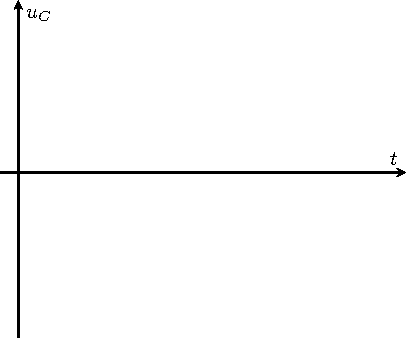
\includegraphics[width=\linewidth]{carac-rlc_empty}
		}{%
			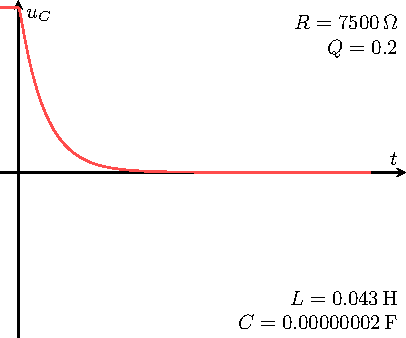
\includegraphics[width=\linewidth]{carac-rlc-02}
		}%
		\vspace{-15pt}
		\captionof{figure}{}
	\end{center}
\end{tcb*}

\begin{tcb}[sidebyside, righthand ratio=.3]
	(inte)<lftt>"bulb"{Espace des phases apériodique}
	Pendant le régime apériodique, l'amortissement est suffisamment important pour
	non seulement empêcher $u_C$ d'osciller, mais également pour \textbf{ralentir
		sa diminution }vers $0$. Son trajet se fait donc à une vitesse plus faible,
	c'est-à-dire $\dv{u_C}{t}$ plus petit donc $i$ plus petit.
	\tcblower
	\begin{center}
		\sswitch{%
			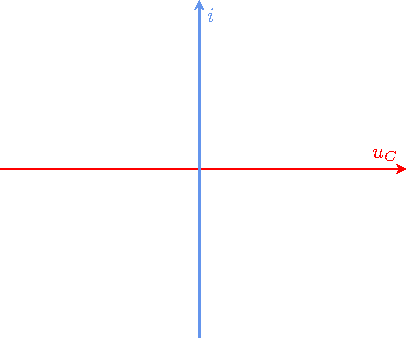
\includegraphics[width=.9\linewidth]{carac-rlc_xy-empty}
		}{%
			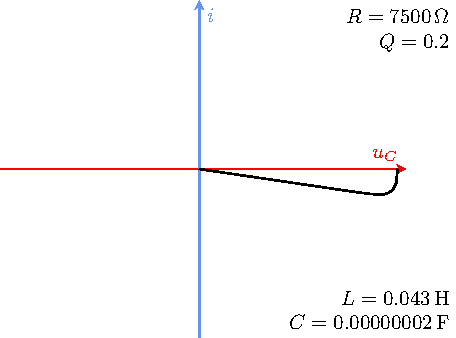
\includegraphics[width=\linewidth]{carac-rlc_xy-02}
		}%
		\vspace{-15pt}
		\captionof{figure}{}
	\end{center}
\end{tcb}

\paragraph{Régime transitoire}
~ \smallbreak

\begin{tcb*}[label=demo:transiaper, breakable](demo){Régime transitoire apériodique}
	La décroissance sera guidée par l'exponentielle la «~\textbf{moins
		décroissante}~». On cherche donc à savoir laquelle, on compare donc $r_-$ et
	$r_+$.
	\smallbreak
	On remarque d'abord que les deux racines sont négatives (d'où la décroissance
	exponentielle)~:
	\begin{isd}
		\vspace{-15pt}
		\psw{%
			\begin{align*}
				r_+ < 0
				 & \Lra
				\underbracket[1pt]{\cancel{-\frac{\w_0}{2Q}}}_{\w_0 \text{ et } Q > 0}
				\left( 1 - \sqrt{1-4Q^2}
				\right) \underbracket[1pt]{\cancel{<}}_{>} 0
				\\&\Lra
				1 - \sqrt{1 - 4Q^2} > 0
				\\&\Lra
				\sqrt{1-4Q^2}^{2} < 1^{2}
				\\&\Lra
				4Q^2 > 0
			\end{align*}
		}%
		ce qui est vrai.
		\tcblower
		Or,
		\vspace{-25pt}
		\psw{%
			\begin{DispWithArrows*}[]
				r_- &< r_+
				\CArrow{$\abs{\cdot}$}
				\\\Lra
				\abs{r_-} &> \abs{r_+}
				\CArrow{$(\cdot)^{-1}$}
				\\\Lra
				\abs{\frac{1}{r_-}} &< \abs{\frac{1}{r_+}}
				\Arrow{$\tau = \abs{1/r}$}
				\\\Lra
				\tau_- &< \tau_+
			\end{DispWithArrows*}
		}%
		On estime alors la durée du régime transitoire à \fbox{$\ln(20)/\abs{r_+}$}.
	\end{isd}
	\bigbreak
	Pour $Q \ll 1$, on utilise \fbox{$\sqrt{1+x} \Sim_{x\ll1} 1+x/2$} pour
	simplifier $r_+$~:
	\psw{%
		\begin{align*}
			r_+ & =
			-\frac{\w_0}{2Q} \left( 1 - \sqrt{1-4Q^{2}} \right)
			\\\Ra
			r_+ & \Sim_{Q\ll1}
			- \frac{\w_0}{2Q} \left( 1 - \left(1 - \frac{4Q^2}{2}\right) \right)
			\\\Lra
			r_+ & \Sim_{Q\ll1} -Q\w_0
		\end{align*}
	}%
	\vspace{-15pt}
	\begin{gather*}
		\beforetext{Avec $\ln(20) \approx \pi$~:}
		\psw{%
			\boxed{t_{95} \approx \frac{\pi}{Q\w_0}}
			\qso
			\boxed{t_{95} \approx \frac{T_0}{2Q}}
		}%
	\end{gather*}
\end{tcb*}

\begin{tcb*}[label=prop:transiaper](prop){Régime transitoire apériodique}
	Le temps de réponse à 95\% est atteint à partir de $t_{95}$ tel que
	\psw{%
		\begin{equation*}
			\boxed{
				t_{95} \approx \frac{T_0}{2Q}} \qav \boxed{T_0 =
				\frac{2\pi}{\w_0}
			}%
		\end{equation*}
	}%
\end{tcb*}

\begin{tcb}[label=impl:aperpetitQ](impl){Résultat à faible $Q$}
	Quand $Q \longrightarrow 0$, on peut négliger le terme d'ordre 2 dans
	l'équation différentielle~:
	\psw{%
		\begin{gather*}
			\frac{\cancel{\w_0}}{Q}\dv{u_C}{t} +
			\w_0{}^{\cancel{2}}u_C = R \sqrt{\frac{C}{L}} \dv{u_C}{t} +
			\frac{1}{\sqrt{LC}}u_C \\
			=
			\dv{u_C}{t} + \frac{1}{R}
			\sqrt{\frac{\bcancel{L}}{\bcancel{L}C^2}} u_C
			=
			\boxed{ \dv{u_C}{t} +
				\frac{1}{RC} u_C}
		\end{gather*}
	}%
	d'où la décroissance exponentielle. D'autre part, les valeurs de $r_\pm$
	tendent vers la même valeur $r = - \frac{\w_0}{2Q}$~: en supposant la solution
	comme la somme des deux racines, on aurait une décroissance~:
	\begin{gather*}
		r = -\frac{\w_0}{Q} = - \frac{1}{\sqrt{LC}}R
		\sqrt{\frac{C}{L}}
		\Lra
		r = -R \sqrt{\frac{\cancel{C}}{L^2\cancel{C}}}
	\end{gather*}
	soit une décroissance exponentielle avec un temps
	caractéristique $\tau = \frac{L}{R}$.
\end{tcb}

\vspace{-15pt}
\section{Exemple amorti mécanique~: ressort + frottements fluides}

\subsection{Présentation}
\begin{tcb*}[label=def:ressortlibre, sidebyside](defi){Situation
			initiale et bilan des forces}
	\begin{itemize}[label=$\diamond$, leftmargin=10pt]
		\item[b]{Système}:
		      \psw{%
			      \{point M\} de masse $m$
		      }%
		      % , accroché à un \textbf{ressort idéal avec frottements}
		\item[b]{Référentiel}:
		      \psw{%
			      $\Rc\ind{sol}$ supposé galiléen
		      }%
		\item[b]{Repère}:
		      \psw{%
			      $(\Or', \ux, \uy)$ (voir schéma)
		      }%
		\item[b]{Repérage}:
		      % \vspace{-15pt}
		      % \begin{center}
		      %  \hspace*{-10pt}
		      %  \fbox{Soit $x (t) = \ell(t) - \ell_0$ la position de la masse}
		      % \end{center}
		      \psw{%
			      \[
				      \hspace{-15pt}
				      \vv{\rm OM} = (\ell(t)-\ell_0)\ux~;
				      \vf = \lp(t)\ux~;
				      \af = \lpp(t)\ux
			      \]
		      }%
		\item[b]{Position initiale}:
		      \psw{%
			      ${\rm OM}(0) = L_0 >0$
		      }%
		\item[b]{Vitesse initiale}:
		      \psw{%
			      $\vf(0) = \of$
		      }%
	\end{itemize}
	\tcblower
	\begin{center}
		\sswitch{%
			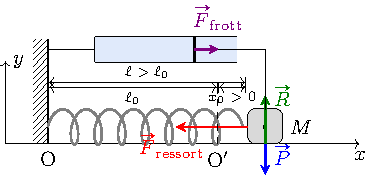
\includegraphics[width=\linewidth, draft=true]{ressort_amorti}
		}{%
			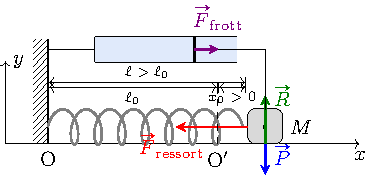
\includegraphics[width=\linewidth]{ressort_amorti}
		}%
		\captionof{figure}{}
	\end{center}
	\begin{itemize}[label=$\diamond$, leftmargin=10pt]
		\item[b]{Bilan des forces~:}
		      \psw{%
			      \[
				      \begin{array}{ll}
					      \textbf{Poids}            & \Pf = m\gf = -mg \uy         \\
					      \textbf{Réaction support} & \Rf = R\uy                   \\
					      \textbf{Force rappel}     & \Ff = -kx (t)\ux             \\
					      \textbf{Force frottement} & \Ff_{\rm frott} = -\alpha\vf
				      \end{array}
			      \]
		      }%
	\end{itemize}
\end{tcb*}

\subsection{Équation différentielle}

\begin{tcb*}[label=demo:solreslibre, sidebyside](demo){Équation ressort amorti}
	Avec le PFD~:
	\psw{%
		\begin{gather*}
			m\af = \Pf + \vv{R} + \Ff\\
			\Lra m\left(
			\begin{array}{c}
					\dv[2]{x}{t} \\
					0
				\end{array}
			\right)
			=
			\left(
			\begin{array}{c}
					-k (\ell(t) - \ell_0) -\alpha v \\
					-mg + R
				\end{array}
			\right)
		\end{gather*}
	}%
	Sur l'axe $\ux$ on trouve donc
	\psw{%
		\begin{DispWithArrows*}
			m \dv[2]{\ell}{t} + \alpha \dv{\ell}{t} + k \ell(t) & =
			k \ell_0
			\CArrow{$\mdiv m$}
			\\\Lra
			\dv[2]{\ell}{t} +
			\frac{\alpha}{m} \dv{\ell}{t} +
			\frac{k}{m} \ell(t)                                 & =
			\frac{k}{m} \ell_0
		\end{DispWithArrows*}
	}%
	\tcblower
	On identifie $\w_0$ et $Q$~:
	\psw{%
		\begin{gather*}
			\w_0{}^2 = \frac{k}{m}
			\Lra
			\boxed{\w_0 = \sqrt{\frac{k}{m}}}
			\\\beforetext{et}
			\frac{\alpha}{m} = \frac{\w_0}{Q}
			\Lra
			Q = \frac{m\w_0}{\alpha}
			\Lra
			\boxed{Q = \frac{\sqrt{km}}{\alpha}}
		\end{gather*}
	}%
	\vspace{-15pt}
\end{tcb*}

\begin{tcb*}[label=prop:eqdiffreslibre, sidebyside]
	(prop){Équation ressort amorti}
	La position $x$ de la masse et la longueur $\ell$ du ressort sont régies
	par~:
	\begin{empheq}[box=\fbox]{align*}
		\dv[2]{\ell}{t} +
		\frac{\w_0}{Q} \dv{\ell}{t} + \w_0{}^2\ell(t) &= \w_0{}^2\ell_0
		\\\Lra
		\dv[2]{x}{t} + \frac{\w_0}{Q} \dv{x}{t} + \w_0{}^2x(t) &= 0
	\end{empheq}
	\tcblower
	\begin{itemize}
		\item
		      \psw{%
			      $\DS\boxed{\w_0 = \frac{k}{m}}$ la pulsation propre~;
		      }%
		\item
		      \psw{%
			      $\DS\boxed{Q = \frac{\sqrt{km}}{\alpha}}$ le facteur de qualité.
		      }%
	\end{itemize}
	$\ell_0$ \textbf{reste} donc la longueur d'équilibre du système.
\end{tcb*}

\begin{tcb}[sidebyside, righthand ratio=.35]
	(ror)<lftt>{Analogie RLC-ressort amorti}
	Ici aussi, les deux systèmes sont \textbf{régis par la même équation
		différentielle}. On observe une \textbf{oscillation amortie} du ressort
	autour d'une position d'équilibre, ici $x\ind{eq}=0 \Lra \ell\ind{eq} =
		\ell_0$.
	\bigbreak
	Ici, c'est le coefficient de frottements $\alpha$ qui dissipe~: on l'associe à
	$R$.
	\smallbreak
	\tcblower
	% \captionof{table}{Correspondances}
	\centering
	\begin{tabular}{c@{$\longleftrightarrow$}c}
		\toprule Méca              & Élec                        \\
		\midrule
		\psw{$x$}                  & \psw{$q$}
		\\
		\psw{$v$}                  & \psw{$i$}
		\\
		\psw{$m$}                  & \psw{$L$}
		\\
		\psw{$k$}                  & \psw{$C^{-1}$}
		\\
		\psw{$\sqrt{\frac{k}{m}}$} & \psw{$\frac{1}{\sqrt{LC}}$}
		\\
		\psw{$\alpha$}             & \psw{$R$}
		\\
		\bottomrule
	\end{tabular}
\end{tcb}

\subsection{Bilan énergétique}

\begin{tcbraster}[raster columns=2, raster equal height=rows]
	\begin{tcb}[label=prop:emecacons,
			list entry={\lte\theprop~:~Bilan de puissance ressort}
		](prop){$\Pc$ ressort}
		Dans le système masse-ressort horizontal avec frottements fluides,
		l'énergie mécanique diminue progressivement proportionellement au
		coefficient de friction $\alpha$~:
		\psw{%
			\begin{equation*}
				\boxed{\dv{\Ec_{m}}{t} = -\alpha v^2}
			\end{equation*}
		}%
	\end{tcb}
	\begin{tcb}[label=demo:emecacons
		list entry={\lte\thedemo~:~Bilan de puissance ressort}
		](demo)'r'{$\Pc$ ressort}
		À partir du PFD $\times v$~:
		\psw{%
			\begin{gather*}
				m \dv[2]{x}{t} \dv{x}{t} + \alpha \dv{x}{t} \dv{x}{t} + kx \dv{x}{t} = 0\\
				\Lra \dv{}{t} \left( \frac{1}{2}m \left( \dv{x}{t} \right)^2 +
				\frac{1}{2}kx^2 \right) = - \alpha v^2
			\end{gather*}
		}%
		On a bien $\Ec_m = \Ec_C + \Ec_{p, \rm el}$ qui diminue.
	\end{tcb}
\end{tcbraster}

\subsection{Solutions}
\begin{center}
	\begin{tcb}[label=prop:ressortsolu](prop){Solutions ressort}
		\begin{center}
			\textbf{On a les mêmes solutions en changeant $u_C$ par $x$ et $E$
				par $x_0$}
		\end{center}
	\end{tcb}
\end{center}

\subsection{Résumé oscillateurs amortis}
\begin{tcb}[label=ror:resumeamorti, tabularx={Y|Y|Y}](ror)
	{Résumé -- pas de par cœur~!}
	\vspace{8pt}
	\textbf{Pseudo-périodique} &
	\vspace{8pt}
	\textbf{Critique} &
	\vspace{8pt}
	\textbf{Apériodique}
	\\\hline
	$\D < 0 \Lra Q > 1/2$ & $\D = 0 \Lra Q = 1/2$ & $\D >
		0 \Lra Q < 1/2$
	\\\hline
	\begin{equation*}
		r_\pm = \psw{- \frac{\w_0}{2Q} \pm \jj\W}
	\end{equation*}
	\begin{equation*}
		\W = \psw{\frac{\w_0}{2Q}\sqrt{4Q^{2} - 1}}
	\end{equation*}
	&
	\begin{equation*}
		r = \psw{-\frac{\w_0}{2Q} = -\w_0}
	\end{equation*}
	&
	\begin{equation*}
		r_\pm = \psw{\frac{\w_0}{2Q}\left(-1 \pm \sqrt{1 - 4Q^2}\right)}
	\end{equation*}
	\\\hline
	\begin{gather*}
		u_C(t) = \psw{E\exp \left( -\frac{\w_0}{2Q}t \right)\times}
		\\
		\hspace*{-3pt}
		\psw{%
			\left[
				\cos(\Wt) + \frac{1}{\sqrt{4Q^2 - 1}}\sin(\Wt)
				\right]
		}%
	\end{gather*}
	&
	\begin{gather*}
		u_C(t) = \psw{E(\w_0t + 1) \exp(-\w_0t)}
	\end{gather*}
	&
	\begin{gather*}
		u_C(t) = \psw{\frac{E}{r_+-r_-}\times}
		\\
		\psw{\big(r_+\exp(r_-t) - r_-\exp(r_+t) \big)}
	\end{gather*}
	\\\hline
	$t_{95} \approx \psw{QT_0}$ &
	\[t_{95} \approx \psw{\frac{T_0}{2}}\] &
	\[t_{95} \approx \psw{\frac{T_0}{2Q}}\]
	\\\hline
	\sswitch{%
		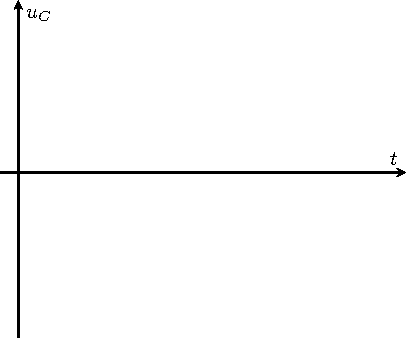
\includegraphics[width=\linewidth]{carac-rlc_empty}
	}{%
		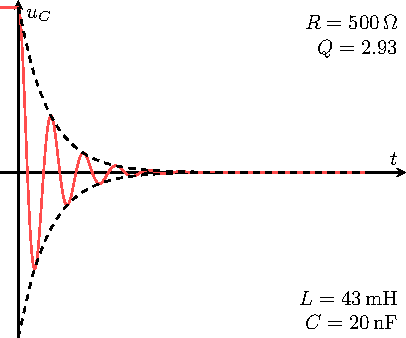
\includegraphics[width=\linewidth]{carac-rlc-3}
	}%
	&
	\sswitch{%
		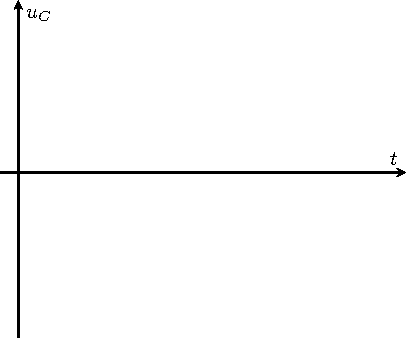
\includegraphics[width=\linewidth]{carac-rlc_empty}
	}{%
		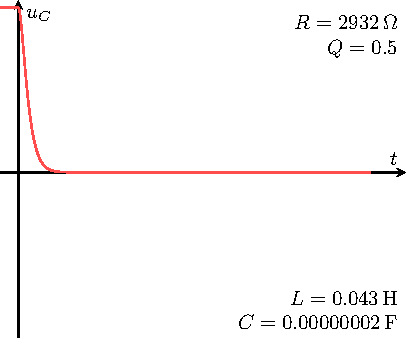
\includegraphics[width=\linewidth]{carac-rlc-05}
	}%
	&
	\sswitch{%
		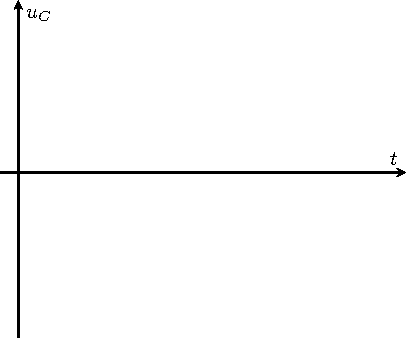
\includegraphics[width=\linewidth]{carac-rlc_empty}
	}{%
		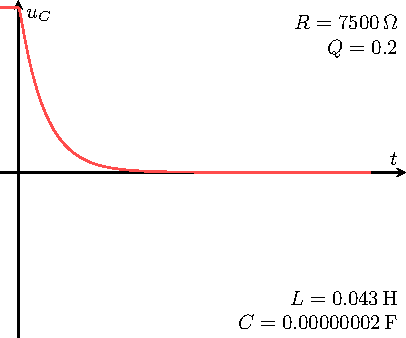
\includegraphics[width=\linewidth]{carac-rlc-02}
	}%
	\\\hline
	\sswitch{%
		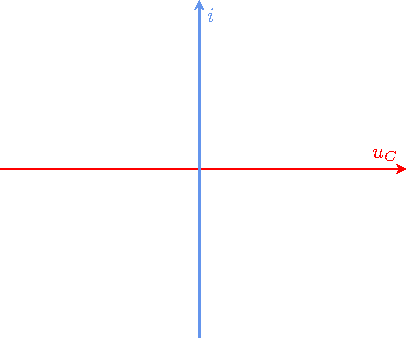
\includegraphics[width=\linewidth]{carac-rlc_xy-empty}
	}{%
		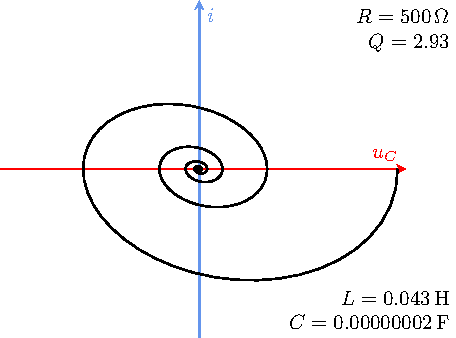
\includegraphics[width=\linewidth]{carac-rlc_xy-3}
	}%
	&
	\sswitch{%
		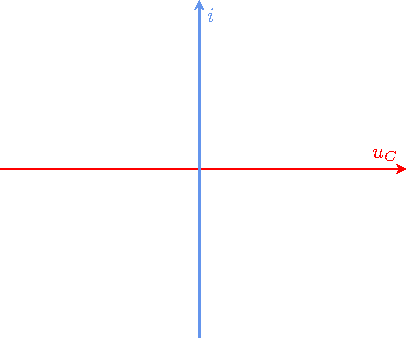
\includegraphics[width=\linewidth]{carac-rlc_xy-empty}
	}{%
		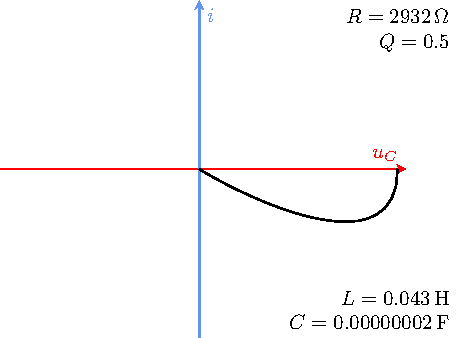
\includegraphics[width=\linewidth]{carac-rlc_xy-05}
	}%
	&
	\sswitch{%
		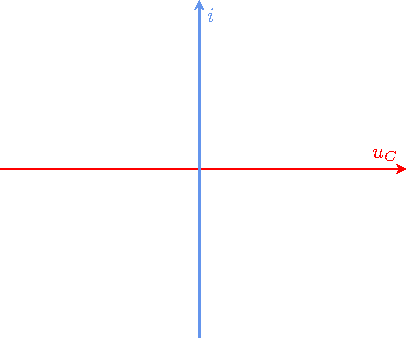
\includegraphics[width=\linewidth]{carac-rlc_xy-empty}
	}{%
		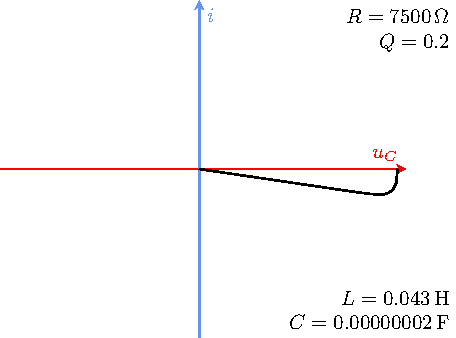
\includegraphics[width=\linewidth]{carac-rlc_xy-02}
	}%
\end{tcb}

\end{document}
